\documentclass[12pt]{article} % use larger type; default would be 10pt

\usepackage{pgfplots}
\usetikzlibrary{calc}
\usetikzlibrary{arrows}
\usetikzlibrary{patterns}
\usetikzlibrary{calc,intersections,through,backgrounds}
\usetikzlibrary{decorations.pathreplacing}
        \usepackage{xcolor} 
        \newcommand\degree[0]{^{\circ}}
        \newcommand\abs[1]{\left|#1\right|}
\usepackage{amsmath}
        \newcommand{\alert}[1]{\boldsymbol{\color{magenta}{#1}}}
        \newcommand{\blert}[1]{\boldsymbol{\color{blue}{#1}}}

\title{Play with TikZ}
\author{Just Us}
%\date{} % Activate to display a given date or no date (if empty),
         % otherwise the current date is printed 

\begin{document}
\maketitle

\section{Chap 8 Section 1}




fig-8-1-ex3


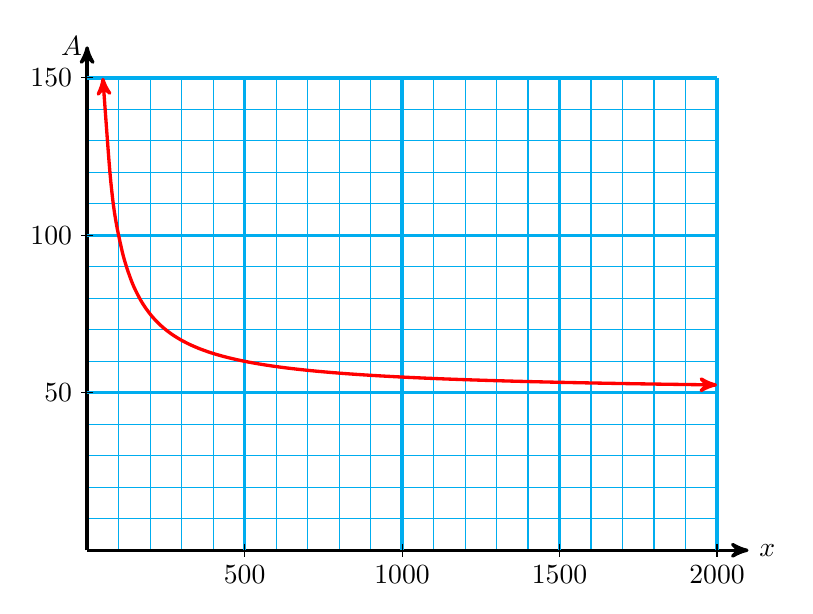
\begin{tikzpicture}[scale=.4]
\draw[cyan] (0,0) grid (20,15);
\draw[black, very thick, ->, >=stealth'] (0,0)--(21,0) node[right]{$x$};
\draw[black, very thick, ->, >=stealth'] (0,0)--++(0,16) node[left, xshift=2]{$A$};
\foreach \x [evaluate=\x as \xi using int(100*\x)] in  {5,10,15,20} {
 \draw[cyan, very thick] ({\x},0) --++(0,15);
 \draw[black] ({\x},.2) --++(0,-.4) node[below, yshift=-2, fill=white, inner sep=1]   {$\xi$};
}
\foreach \x [evaluate=\x as \xi using int(10*\x)] in  {5,10,15} {
 \draw[cyan, very thick] (0,\x) --++(20,0);
 \draw[black] ({.2},\x) --++(-.4,0) node[left, xshift=-2, fill=white, inner sep=1]   {$\xi$};
}
\draw[samples=65,domain=1/2:20,smooth,variable=\x,red, very thick,<->, >=stealth'] plot ({\x},{(5 + 5*\x) / \x});
\end{tikzpicture}
\newline


hp-8-1-46 grid


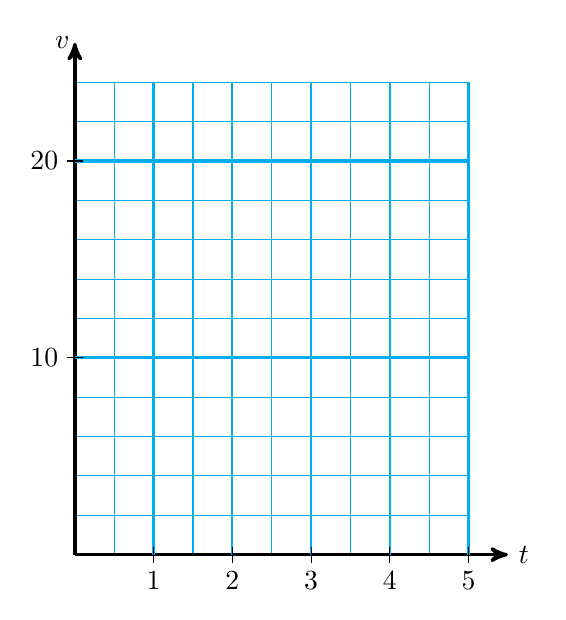
\begin{tikzpicture}[scale=.5]
\draw[cyan] (0,0) grid (10,12);
\draw[black, very thick, ->, >=stealth'] (0,0)--(11,0) node[right]{$t$};
\draw[black, very thick, ->, >=stealth'] (0,0)--++(0,13) node[left, xshift=2]{$v$};
\foreach \x  [evaluate=\x as \xi using int(1/2*\x)] in  {2,4,6,8,10} {
 \draw[cyan,  thick] ({\x},0) --++(0,12);
 \draw[black] ({\x},.2) --++(0,-.4) node[below, yshift=-2, fill=white, inner sep=1]   {$\xi$};
}
\foreach \x [evaluate=\x as \xi using int(2*\x)] in  {5,10} {
 \draw[cyan, very thick] (0,\x) --++(10,0);
 \draw[black] ({.2},\x) --++(-.4,0) node[left, xshift=-2, fill=white, inner sep=1]   {$\xi$};
}
\end{tikzpicture}
\newline



hp-8-1-47 grid


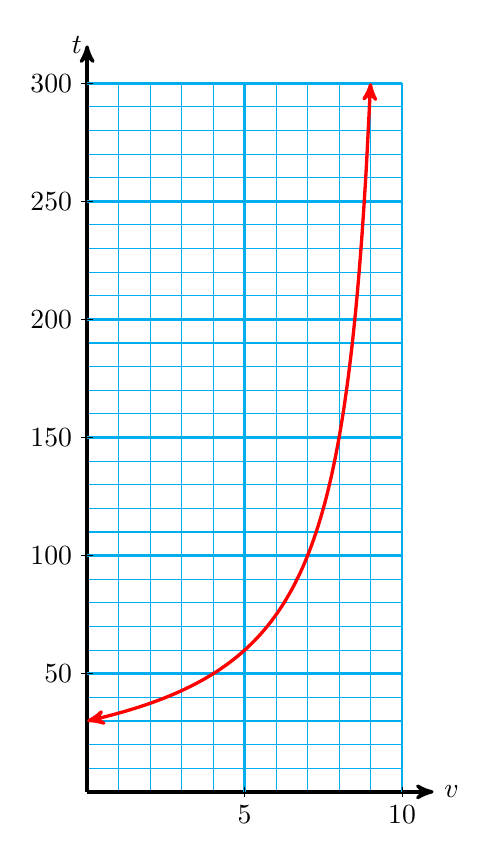
\begin{tikzpicture}[xscale=.4, yscale=.3]
\draw[cyan] (0,0) grid (10,30);
\draw[black, very thick, ->, >=stealth'] (0,0)--(11,0) node[right]{$v$};
\draw[black, very thick, ->, >=stealth'] (0,0)--++(0,31.6) node[left, xshift=2]{$t$};
\foreach \x in  {5,10} {
 \draw[cyan,  thick] ({\x},0) --++(0,30);
 \draw[black] ({\x},.2) --++(0,-.4) node[below, yshift=-2, fill=white, inner sep=1]   {$\x$};
}
\foreach \x [evaluate=\x as \xi using int(10*\x)] in  {5,10, 15,...,30} {
 \draw[cyan, very thick] (0,\x) --++(10,0);
 \draw[black] ({.2},\x) --++(-.4,0) node[left, xshift=-2, fill=white, inner sep=1]   {$\xi$};
}
\draw[samples=65,domain=0:9,smooth,variable=\x,red, very thick,<->, >=stealth'] plot ({\x},{30 / (10-\x)});
\end{tikzpicture}
\newline


fig-8-2-1 colored rectangles

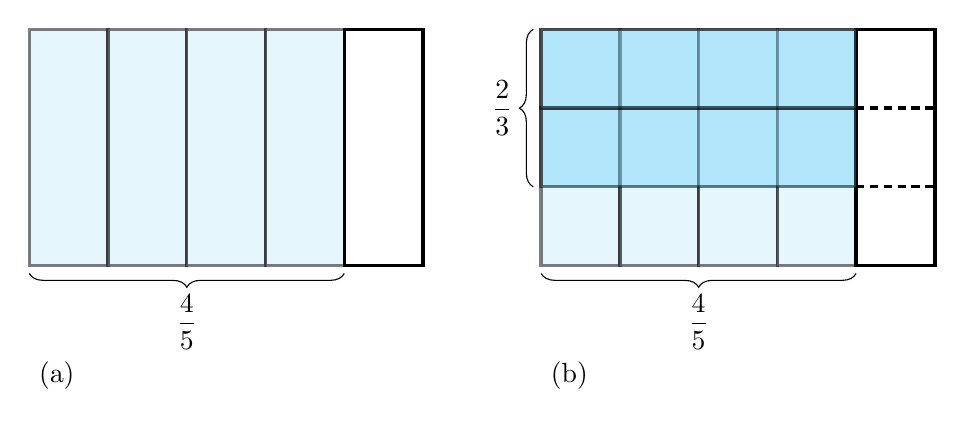
\begin{tikzpicture} 
\foreach \x in {0,1,2,3} {
 \draw[black, fill=cyan!20!white, very thick, opacity=.5] (\x,0) rectangle ++(1,3);
}
\draw[black, very thick] (4,0) rectangle ++(1,3);
\draw [black,decorate,decoration={brace,amplitude=5pt}] (4,0)++(0, -.1) -- ++(-4,0) node [black, below,midway,yshift=-4pt] {$\displaystyle\frac{4}{5}$};

\coordinate(A) at (6.5,0);
\foreach \x in {0,1,2,3} {
 \draw[black, fill=cyan!20!white, very thick, opacity=.5] (A)++(\x,0) rectangle ++(1,3);
}
\draw[black, very thick] (A)++(4,0) rectangle ++(1,3);
\draw [black,decorate,decoration={brace,amplitude=5pt}] ($ (A)+(4,0)+(0, -.1)$) -- ++(-4,0) node [black, below,midway,yshift=-4pt] {$\displaystyle\frac{4}{5}$};
\foreach \x in {1,2} {
 \draw[black, fill=cyan!50!white, very thick, opacity=.5] (A)++(0,\x) rectangle ++(4,1);
 \draw[black,very thick, densely dashed] (A)++(4,\x)--++(1,0);
}
\draw [black,decorate,decoration={brace,amplitude=5pt}] ($ (A)+(0,1)+(-.1,0)$) -- ++(0,2) node [black, left,midway,xshift=-4pt] {$\displaystyle\frac{2}{3}$};
\node[right] at (0,-1.4) {(a)};
\node[right] at ($(A)+(0,-1.4)$) {(b)};
\end{tikzpicture}
\newline



fig-8-2-2 rectangles

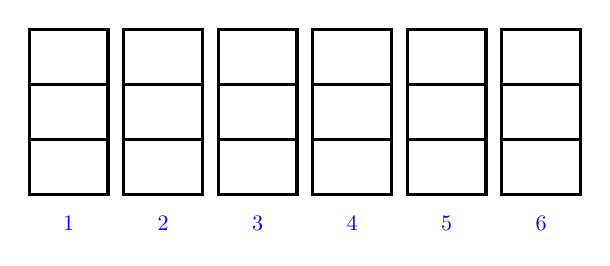
\begin{tikzpicture} 
\foreach \x in {1,2,3,...,6} {
 \draw[black, very thick] ({1.2*\x-.5},0) rectangle ++(1,2.1);
 \draw[black, thick] ({1.2*\x-.5},0.7)--++(1,0);
 \draw[black, thick] ({1.2*\x-.5},1.4)--++(1,0);
 \node[text=blue, scale=.8] at ($1.2*(\x,-.3)$) {\x};
}
\end{tikzpicture}
\newline




\section{Section 8.3}



fig-8-3-1a subdivided rectangle

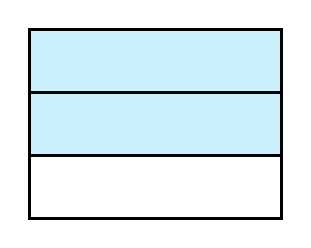
\begin{tikzpicture} [scale=.8]
\foreach \x in {1,2} {
 \draw[black, fill=cyan!20!white, very thick] (0,\x) rectangle ++(4,1);
}
\draw[black, very thick] (0,0) rectangle ++(4,1);

\end{tikzpicture}
\newline


fig-8-3-1b subdivided rectangle

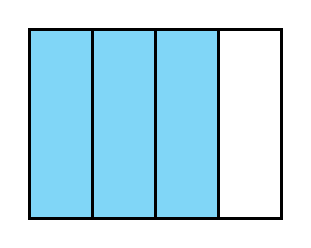
\begin{tikzpicture} [scale=.8]
\foreach \x in {0,1,2} {
 \draw[black, fill=cyan!50!white, very thick] (\x,0) rectangle ++(1,3);
}
\draw[black, very thick] (3,0) rectangle ++(1,3);
\end{tikzpicture}
\newline



fig-8-3-2a subdivided rectangle

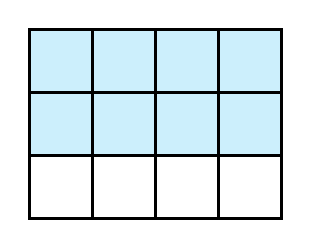
\begin{tikzpicture} [scale=.8]
\foreach \x in {1,2} {
 \draw[black, fill=cyan!20!white, very thick] (0,\x) rectangle ++(4,1);
}
\draw[black, very thick] (0,0) rectangle ++(4,1);
\foreach \x in {1,2,3} {
 \draw[black, very thick] (\x,0) --++(0,3);
+(1,3);
}

\end{tikzpicture}
\newline


fig-8-3-2b subdivided rectangle

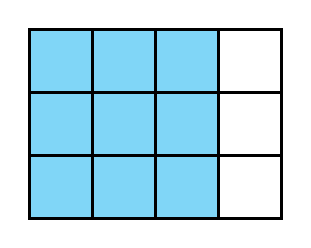
\begin{tikzpicture} [scale=.8]
\foreach \x in {0,1,2} {
 \draw[black, fill=cyan!50!white, very thick] (\x,0) rectangle ++(1,3);
}
\draw[black, very thick] (3,0) rectangle ++(1,3);
\foreach \x in {1,2} {
 \draw[black, very thick] (0,\x) --++(4,0);
}
\end{tikzpicture}
\newline




\section{Section 8.4}



hp-8-4-23 golden rectangle

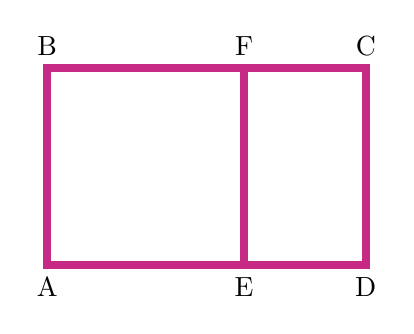
\begin{tikzpicture} [scale=2.5]
\def\r{(1+sqrt(5))/2};
\draw[magenta!80!black,  line width=1mm] (0,0) rectangle ++({\r},1);
\draw[magenta!80!black,  line width=1mm] (1,0) --++(0,1);
\node [below, yshift=-1] at (0,0) {A};
\node [below, yshift=-1] at (1,0) {E};
\node [below, yshift=-1] at ({\r},0) {D};
\node [above, yshift=1] at (0,1) {B};
\node [above, yshift=1] at (1,1) {F};
\node [above, yshift=1] at ({\r},1) {C};
\end{tikzpicture}
\newline







\section{Other stuff}

10 by 10 grid: hp-2-3-12

8 by 8 grid: hp-4-5-17



\end{document}
